\section{Introduction}

A drug that reaches the bloodstream does not remain the compound that was administered. Enzymes,
predominantly hepatic, convert it into other compounds, and those compounds carry activity,
toxicity and persistence of their own. Some of them are the species that acts: the antiviral
prodrugs are inactive as administered and reach their target only after phosphorylation
\citep{To_2023}. Others end a development programme, as the reactive intermediate implicated in
the withdrawal of troglitazone did \citep{Ikeda_2011}. Knowing which compounds an enzyme system
will make from a candidate drug therefore belongs with the properties a medicinal chemist asks
about early.

Experimental metabolite identification answers the question for a compound that has been
synthesised and dosed. A computational prediction is available earlier, while a compound exists
only as a drawing, and that is when its structure can still be changed in response. The
prediction asked for here is the chemical structure of each metabolite, which is a harder object
than the quantities usually predicted alongside it. A clearance rate is a number and a site of
metabolism is an atom, whereas a metabolite is a molecular graph that has to be correct bond by
bond; a proposal that is chemically reasonable but constitutionally wrong is of no use to the
chemist who would synthesise it.

Two families of method are in use. Rule-based systems encode known biotransformations as reaction
templates, patterns that match a substructure of the substrate and rewrite it, and they enumerate
the products of applying those templates. SyGMa \citep{Ridder_2008}, BioTransformer
\citep{Djoumbou_Feunang_2019}, GLORY and GLORYx \citep{de_Bruyn_Kops_2019, de_Bruyn_Kops_2020} and
MetaTox \citep{Rudik_2017} are of this kind. Sequence-to-sequence systems treat the problem as
translation between string representations of the substrate and of its metabolites, and MetaTrans
\citep{Litsa_2020} and MetaPredictor \citep{Zhu_2024} are of this kind. Both lines have been
extended recently \citep{Larsson_2025, Zhou_2025, Zhou_2026, Chavan_2026}. The two families are
used for different reasons. A template names the transformation it applied and the atoms it acted
on, so a chemist can see on what grounds a structure was proposed and can reject it mechanistically;
that property is what makes rule-based systems usable in a discovery workflow. A sequence model
reports the structure alone, and is valued for reaching chemistry that lies outside any template
bank.

Choosing between the two families, or between systems within one of them, requires a comparison
that the published literature does not presently support. The usual measure is recall: of the
metabolites recorded for a compound, the fraction that a system returns. That fraction depends on
two decisions taken outside the model. The first is when a returned structure counts as one of the
recorded metabolites, since two structures can denote the same molecule while differing in the
placement of a hydrogen or the drawing of a ring. The second is how many structures a system is
permitted to return, since any system recovers more of the answer when allowed a longer list.
Published predictors differ on both decisions and report them inconsistently. The systems compared
here return between \numWholeemitMin{} and \numWholeemitMax{} structures per substrate under their
default settings, so their recall figures sit on different scales. Independent
evaluations of these tools have encountered the same obstacle
\citep{Boyce_2022, Scholz_2023, Gao_2026}.

That a comparison can turn on an undeclared choice has been argued before, and two recent
statements of it bound what the present work adds. \citet{Ash_2025} set out a protocol for method
comparison in small-molecule drug discovery, arguing that a difference should be shown practically
significant and prescribing how such a comparison ought to be constructed. \citet{Ozcelik_2025}
show what follows when it is not, in generative molecular design, where the size of the library
and the choice of metric reorder the models. The multiverse and specification-curve literature
\citep{Steegen_2016, Simonsohn_2020} reports results across the whole space of defensible analysis
choices, and the present work applies that discipline to metabolite structure prediction. A protocol tells an
author what to declare. Generative metrics are distributional, and the axis that reorders methods
here, the number of candidates a system may emit, belongs to ranked output alone, so recall
against an incomplete annotation needs its own demonstration.

We report GRAIL (Graph-scored Rule Application with Inspectable Localisation), a predictor of
metabolite structures assembled from a bank of reaction templates, a learned model that selects
which templates to apply to a given substrate, and a learned model that ranks the structures those
templates produce. GRAIL is the engine of MetaTox~3.0 at \texttt{way2drug.com}, replacing MetaTox
\citep{Rudik_2017} as the predictor that service answers with; Section~\ref{sec:results} compares
the two. We evaluate GRAIL with both of the decisions above raised to
declared axes, each named and each swept across its full range, against
\numComparatorsColumnsWord{} published predictors we obtained and ran ourselves on one common set
of drug-like substrates. This paper leaves three
things behind it. The first is the comparison as data: the per-substrate predictions of all
\numArmsTotalWord{} arms on the \numWholeN{} substrates, frozen and released with the harness that
scores them, so any cell of any table here can be recomputed and any later system added to the
same grid under the same two axes. For want of such a set, the orderings in this literature are at
present checkable only by their authors. The second is a bound: one application of the whole bank
reaches \numCeilingCoverage{} of known metabolites in a single step, and a census of what it
misses says which chemistry is absent and where to look for it, which holds of every bank mined
from the sources this field trains on. The third is what the bank is made of:
\numThirdpartyBorrowedsharePct{} of its curated templates appear verbatim in rule sets published
by others, so what this work contributes to it is the mining, and the mined half is what carries
the chemistry in the worked example of Section~\ref{sec:cases}.



\section{Materials and methods}
\label{sec:methods}

\subsection{Corpus, splits and evaluation populations}
\label{sec:populations}

The corpus is assembled from ChEMBL \citep{Zdrazil_2024}, DrugBank \citep{Wishart_2018},
MetXBioDB \citep{Djoumbou_Feunang_2019} and the GLORYx reference set
\citep{de_Bruyn_Kops_2020}, at versions \CorpusVersions{}. Each record pairs a substrate with one
metabolite reported for it, and we call that metabolite a \emph{known metabolite} throughout. The
corpus divides into three splits that share no substrate, as a held-out figure requires
\citep{Joeres_2025, Kretschmer_2025}: \numSplitTrainSubstrates{} substrates for training,
\numSplitValSubstrates{} for validation and \numSplitTestSubstrates{} for testing, carrying
\numSplitTrainPairs{}, \numSplitValPairs{} and \numSplitTestPairs{} annotated pairs respectively.

Three populations carry the figures, and every figure names the one it is measured on. The
\emph{evaluated test set} is every test substrate with a known metabolite, \numWholeN{} of them
carrying \numWholeReferences{} known metabolites. It carries every
comparison against a published predictor and the coverage bound of Section~\ref{sec:ceiling}. The \emph{validation draw} is a declared sample of the validation split, on which the
preregistered thresholds of Section~\ref{sec:register} are checked, since a threshold has to be checked on
a population other than the one that chose the setting. The
\emph{comparison set} is the \numPopulationN{} substrates submitted to the one comparator that
runs as a web service, carrying \numPopulationReferences{} known metabolites. A column of a
comparison is an \emph{arm}, and this system contributes two, described in
Section~\ref{sec:modes}.

That set records which substrates were submitted, not which were answered: every method has an
entry for all of them. The rule by which the list was drawn was not recorded, so it carries a
selection nobody here can describe. It is kept because the controls were computed on it: matched list
length, the matching criterion, the transformation classes, precision and the parent-drop
convention. The sweep runs on both populations, so the move can be read cell by
cell.

\subsection{The predictor}

GRAIL works in three stages, and each can be inspected on its own. A \emph{generator} scores every
rule in a bank of reaction templates against the substrate and selects which of them to apply. The selected rules
are then applied with RDKit, and their products are standardised \citep{Hahnke_2018,
Mansouri_2024} and deduplicated. A rule that breaks a bond yields more than one product, and every
product and every disconnected component of one enters separately provided it
retains at least \numFragmentFloorWord{} heavy atoms, which discards a lone leaving group while
keeping a small metabolite such as formate. A surviving product is a \emph{candidate}, and the
candidates generated for one substrate are its \emph{pool}. Finally a \emph{scorer} evaluates each
substrate--candidate pair, encoding the two molecules in separate molecular graphs, and the pool is
ordered by a fusion of the scorer's ranking with the generator's.

The bank holds \numBankRules{} templates spanning \numBankTypes{} reaction types, where a type is
the multiset of bonds that change between mapped atoms. A template is a mapped SMIRKS pattern, and
we use \emph{rule} for the same object here and in the released files. The bank is the deduplicated
union of \numAttribNamed{} templates from three curated collections, \numMinedRules{} mined from
the training split alone, and \numAttribUnattributed{} that an earlier machine extraction took from
the same annotated pairs. At least \numThirdpartyBorrowed{} of the \numAttribNamed{} curated
templates, \numThirdpartyBorrowedsharePct{}, appear verbatim in rule sets published by others,
so this work's contribution is the mining, the ranking and the measurement. Support across the mined templates is heavily
skewed, with \numRareSingletonsharePct{} of them resting on a single training pair, and a
rarefaction curve over withheld pairs is still climbing, so this corpus still yields
templates that are new.

Several rules, or one rule firing at several sites, can reach the same candidate, and such a
candidate receives a single score. Writing $R(c)$ for the rules that produce candidate $c$ and
$p_r$ for the generator's probability that rule $r$ applies, we combine them by noisy-or,
\begin{equation}
p(c) = 1 - \prod_{r \in R(c)} \left( 1 - p_r \right),
\label{eq:noisyor}
\end{equation}
so that independent rules reinforce one another. Independence is an
assumption this bank does not satisfy, since it holds published rule sets verbatim and its mined
half contains many near-duplicates, and we therefore sweep the four aggregation rules the
implementation offers.

Both learned stages hold an opinion about every candidate, and multiplying the two is sensitive to
their scales: if one scorer occupies a narrow range and the other a wide one, the wide one decides
the order. We combine them instead by reciprocal rank fusion \citep{cormack2009}, which scores a
candidate as the sum over the two scorers of $1/(K + r)$ with $r$ its rank under that scorer. Only
positions enter, so the two opinions contribute equally whatever their scales. We use the published
value $K = \numFusionkDeployed$ and sweep it as well as declaring it. Before the fusion, the pool
is truncated by generator score, a quantity available before any pair graph is built,
\begin{equation}
\hat{C}(s) = \operatorname*{arg\,top}_{c \in C(s)}{}^{\,\numHNineCap} \; p(c),
\end{equation}
where $C(s)$ is everything the applied rules enumerate. Because the fusion ranks over whatever
survives, removing a candidate changes the rank of every other, and truncation can raise recall as
well as bound it. We set the cap at twice the widest output budget reported, so that the widest
column of a comparison is never simply the whole pool.

How many templates the generator selects before any is applied is the \emph{rule budget}. It is not the output budget of Section~\ref{sec:evaluation}, which is how many candidates a system may return; where this paper writes \emph{budget} unqualified it means that one. The rule budget
sets the two operating modes the service offers.

\subsubsection{Operating modes}
\label{sec:modes}

The \emph{interactive} mode applies the \numHOneZeroTopk{} templates the trained checkpoint
records and answers in about a second, which is what a user waiting at a web form requires. The
\emph{exhaustive} mode applies the whole bank, the \numBankParses{} templates of
\numBankRules{} that parse, and takes tens of seconds. Table~\ref{tab:modes} gives what each mode
returns and recovers on the validation draw.

\begin{table}[t]
\centering\footnotesize
\begin{threeparttable}
\caption{The two operating modes: rules applied, candidates returned and wall-clock time.}
\label{tab:modes}
\begin{tabular}{lrr}
\toprule
 & interactive & exhaustive \\
\midrule
rules applied & 30 & 7{,}580 \\
candidates, mean & 16.5 & 98.0 \\
candidates, median & 14.0 & 100 \\
seconds, median & 0.39 & 5.28 \\
seconds, mean & 2.36 & 52.77\tnote{a} \\
seconds, 90th pct & 2.59 & 89.78\tnote{a} \\
seconds, slowest & 231.01 & $>600$\tnote{a} \\
\bottomrule
\end{tabular}
\begin{tablenotes}[flushleft]\footnotesize
\item Every unmarked row is measured on the validation draw, 294 substrates for the
interactive mode and 293 for the exhaustive one. Candidates are what a caller
receives, deduplicated by matching key and capped at 100. Times cover
everything before the filter.
\item[a] Taken over a sampled timing sweep of 106 substrates and censored at a
600-second deadline, which the exhaustive mode exceeds for 11 of them.
\end{tablenotes}
\end{threeparttable}
\end{table}


A rank fusion carries positions alone, so a threshold tuned on a score product loses its meaning: at the value this system registered it admits \numEmitByfusion{} candidates of a pool of \numEmitPool{}. What each mode returns is therefore the capped pool itself, ordered by the
fusion and cut by no threshold. For the interactive mode the length of that list follows from the
rule budget and the substrate's chemistry, and averages \numEmittedTrained{} candidates on the
comparison set, well inside any cap. For the exhaustive mode it averages \numEmittedBank{}, close
enough to the cap that the cap sets the length on most substrates. Emitting the whole pool was
fixed as a prediction and confirmed (Table~\ref{tab:hyp}), on a budget ladder fixed at the same
time, which differs from the ladder read elsewhere here. The binding cost of the whole
pipeline is product standardisation, run once for every product of every template, and two
preregistered changes addressed it.

\subsection{Evaluation protocol}
\label{sec:evaluation}

Whether a returned structure counts as one of the known metabolites is settled by the
\emph{matching criterion}, which we treat as a declared axis with five settings and report under
all five. The tautomer-aware key is the
default, because the known metabolites are recorded as constitutions with tautomers
merged, and because standard identifiers normalise only a subset of tautomers
\citep{Dhaked_2020}. Recording constitutions alone also bounds what these systems can be asked
for: this pipeline works at the level of constitution throughout, so sulfoxidation, epoxide
hydrolysis and most conjugation are predicted with configuration left open.

A third choice sits behind both declared axes: how the substrate itself is drawn. Templates are
matched against the structure the corpus stores, and that corpus draws amides as imidic acids, so
the choice is not neutral. Rebuilding both GRAIL arms with every substrate redrawn moves
\numDsweepMoved{} of \numDsweepCells{} arm-against-comparator verdicts, none of them a result
claimed here.

The number of candidates a system may return is the \emph{output budget}, written $k$, and it is
the second declared axis. Recall at budget $k$ for substrate $s$ with known metabolites $Y_s$ and
the first $k$ predictions $\hat{Y}^{(k)}_s$ is $|Y_s \cap \hat{Y}^{(k)}_s| / |Y_s|$. We distinguish
two aggregations throughout and never mix them within one comparison,
\begin{align}
\mathrm{macro} &= \frac{1}{|S|}\sum_{s \in S}
\frac{|Y_s \cap \hat{Y}^{(k)}_s|}{|Y_s|}, \\
\mathrm{micro} &= \frac{\sum_{s} |Y_s \cap \hat{Y}^{(k)}_s|}{\sum_{s} |Y_s|},
\end{align}
and every figure states which it carries. Intervals are a paired bootstrap over substrates: for
each of $B = 10\,000$ resamples $S^{(b)}$ drawn with replacement,
\begin{equation}
\delta^{(b)} = \frac{\sum_{s \in S^{(b)}} \left( h^A_s - h^B_s \right)}
{\sum_{s \in S^{(b)}} |Y_s|},
\label{eq:bootstrap}
\end{equation}
with $h^A_s$ and $h^B_s$ the hits of the two arms, and the reported interval is the empirical
$2.5$ and $97.5$ percentiles of $\{\delta^{(b)}\}$.

One comparator is not yet published. GLORYxR is the successor to GLORYx, and what ran is a
pre-publication revision of \texttt{github.com/molinfo-vienna/GLORYxR}, recorded by digest in
Section~\ref{SI-sec:si-comparators}.

Every interval reported here is a per-comparison interval with no family-wise adjustment, and we
report the corrected reading beside it. Holm's correction over the family declared in advance, the
two arms against \numSweepFamilycomparatorsWord{} comparators, leaves \numHolmSurviving{} of the
\numHolmSeparating{} separating cells separating, and applying it instead to every contrast printed
anywhere in this work leaves the wide-budget result and every conclusion drawn from it standing.
A claim that the system leads is made for a cell only where that cell's interval excludes zero, and where an ordering is not established the table says so.

\subsection{Preregistered design decisions}
\label{sec:register}

Every deployed choice is a registered hypothesis with a threshold and a falsification condition,
tested where it was not selected (Table~\ref{tab:hyp}). Ten of the sixteen registered predictions are checked in this work.
Six are confirmed and three failed, each on the falsification condition it was written with; the tenth counts as
a measurement, because its threshold was fixed in advance while its population was chosen
afterwards. The remaining six are registered against work reported elsewhere and are stated with their thresholds, so that a later result on any of them rests on a threshold fixed in advance. Section~\ref{sec:limitations} states which of the six confirmations a stricter
reading leaves undecided.

\begin{table*}[t]
\centering\footnotesize
\begin{threeparttable}
\caption{Every deployed choice as a prediction fixed before it was checked: what was fixed, the threshold, the value measured, the population it was checked on, and what the check returned.}
\label{tab:hyp}
\begin{tabular}{@{}lllllp{0.125\textwidth}l@{}}
\toprule
 & what was fixed & threshold & measured & tested on & verdict & register \\
\midrule
P1 & rank fusion instead of a score product & $+0.05$ & $+0.0733$ & validation & confirmed; threshold inside interval & H7 \\
P2 & candidate pool capped at 100 & $+0.015$ & $+0.0260$ & validation & confirmed; threshold inside interval & H9 \\
P3 & rule budget of 30 & $\le +0.05$ & $+0.0092$ & validation & confirmed on validation; not on the comparison set & H10 \\
P4 & emit the whole pool, no threshold & 0 cells & $0$ & grid $5\times11$ & confirmed & H11 \\
P5 & group score as a third ranking & $+0.02$ & $+0.0256$ & comparison set$^{\dagger}$ & measured, not adjudicated in advance; threshold inside interval & H12 \\
P6 & group score, groups emitted as blocks & $+0.05$ & $-0.1188$ & comparison set$^{\dagger}$ & failed & H8 \\
P7 & group score as a gate before fusion & $+0.02$ & $-0.0195$ & comparison set$^{\dagger}$ & failed & H14 \\
P8 & standardise survivors only & $\ge 10\times$ & $2.95$ & validation & failed & H13 \\
P9 & survivors, tautomer budget 200 & $<10$ s & $5.28$ & validation & confirmed & H15 \\
P10 & composite share, both instruments & $\ge 0.134$ & $0.2212$ & mined bank & confirmed & H16 \\
\bottomrule
\end{tabular}
\begin{tablenotes}[flushleft]\footnotesize
\item P8's figure is a speed-up factor, P9's a median in seconds and P10's a share of the mined bank; the rest are differences in micro recall at a budget of 15. $^{\dagger}$ marks the three whose threshold was fixed in advance but whose population was not. The last column carries each row's identifier in the released register, which numbers the predictions in the order they were written rather than the order they are read.
\end{tablenotes}
\end{threeparttable}
\end{table*}


\section{Results}
\label{sec:results}

\subsection{Comparison with published predictors}

\begin{table*}[t]
\centering
\begin{threeparttable}
\caption{Micro recall at each output budget on the 1170 substrates of the whole evaluated test set, carrying 2597 annotated metabolites.}
\label{tab:sweep}
\scriptsize
\setlength{\tabcolsep}{4.5pt}
\begin{tabular}{rrrrrrrrrr}
\toprule
$k$ & GRAIL exh. & GRAIL int. & MetaTox & SyGMa & MetaPred. & BioTrans. & GLORYx & GLxR d. & GLxR s. \\
\midrule
1 & 0.1070 & 0.1167 & 0.0420 & 0.1533 & 0.1621 & 0.0705 & 0.0836 & 0.0936 & 0.1205 \\
3 & 0.2287 & 0.2472 & 0.1567 & 0.3134 & 0.3123 & 0.1787 & 0.2091 & 0.2333 & 0.2649 \\
5 & 0.3057 & 0.3285 & 0.2499 & 0.4016 & 0.3939 & 0.2514 & 0.3123 & 0.3331 & 0.3577 \\
8 & 0.3962 & 0.4024 & 0.3458 & 0.4575 & 0.4621 & 0.3231 & 0.4193 & 0.4182 & 0.4343 \\
10 & 0.4390 & 0.4394 & 0.4085 & 0.4813 & 0.4840 & 0.3593 & 0.4682 & 0.4605 & 0.4771 \\
15 & 0.5295 & 0.4875 & 0.5075 & 0.5137 & 0.4975 & 0.4186 & 0.5445 & 0.5306 & 0.5306 \\
20 & 0.5834 & 0.5052 & 0.5522 & 0.5268 & 0.4979 & 0.4401 & 0.5845 & 0.5703 & 0.5645 \\
30 & 0.6484 & 0.5144 & 0.6103 & 0.5341 & 0.4979 & 0.4482 & 0.6157 & 0.6057 & 0.5961 \\
50 & 0.7174 & 0.5156 & 0.6438 & 0.5360 & 0.4979 & 0.4486 & 0.6307 & 0.6219 & 0.6203 \\
\midrule
\emph{mean emitted} & \emph{97.94} & \emph{17.07} & \emph{35.70} & \emph{80.73} & \emph{10.61} & \emph{11.08} & \emph{30.70} & \emph{30.52} & \emph{30.52} \\
\bottomrule
\end{tabular}
\begin{tablenotes}[flushleft]\footnotesize
\item The last row gives the mean number of candidates each method emits, before any budget is applied: it is a property of the method and not of this table. These arms emit more than the widest budget shown, 50: GRAIL exh., SyGMa. A prediction equal to the substrate is dropped before the budget for every method alike. Figure~\ref{fig:sweep} plots these recalls and marks the budgets at which the difference from the strongest comparator separates.
\end{tablenotes}
\end{threeparttable}
\end{table*}


Every comparator has an entry for the whole evaluated test set, so the comparison runs there, over
\numWholeN{} substrates and \numWholeReferences{} known metabolites (Table~\ref{tab:sweep}),
scoring zero where one returns nothing. The same sweep over the \numPopulationN{}-substrate
comparison set, the slice one control below uses, is Table~\ref{SI-tab:sweep-comparison}.

We read it first with the budget taken from the comparator, because a nominal budget caps a list
and leaves its length to the system: by $k=30$ most comparator lists have ended, so a difference
read there is partly a difference in how much each emits. Cutting both arms to the comparator's
own realised length on every substrate (Figure~\ref{fig:matched}, Table~\ref{SI-tab:si-matched})
leaves \numMatchedSurviveWord{} of the
\numMatchedComparatorsWord{} wide-budget leads standing, over \numMatchedSurvivenames{}, at
$+\numMatchedBanksygma$ $[+\numMatchedBanksygmaLo, +\numMatchedBanksygmaHi]$ over
\numMatchedBanksygmaSlots{} slots. Of the \numMatchedOthersWord{} that fall,
\numMatchedOthersagainstWord{} settle against this work with the interval excluding zero,
\numMatchedOthersagainstnames{}, and \numMatchedOthersundecidedWord{} stay undecided. One of the undecided
is BioTransformer, which is not the lowest arm at the tight budgets, where MetaTox is, and which
supplies \numThirdpartyBiotransformerShipped{} of this bank's templates. The ordering result is
one comparator wide.

\begin{figure}[t]
\centering
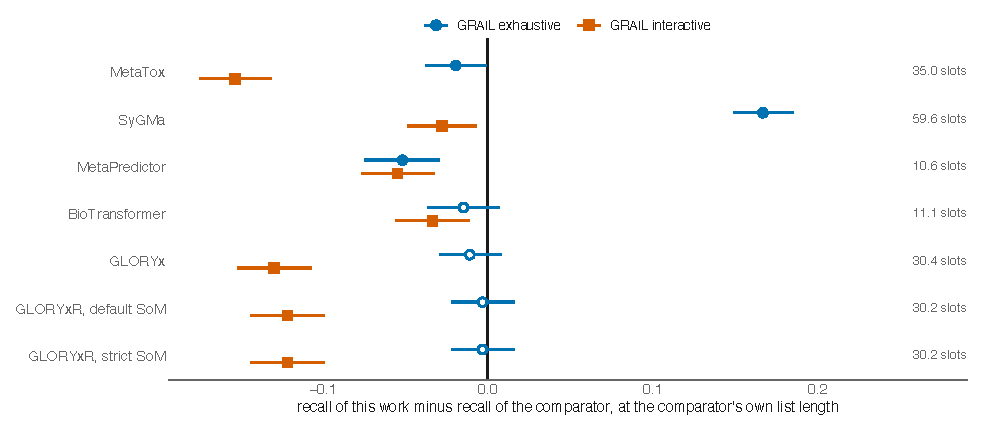
\includegraphics[width=\columnwidth]{fig_matched}
\caption{The comparison with the output budget taken from the comparator, on the \numWholeN{}
substrates of the whole evaluated test set. A mark is the recall of one GRAIL arm minus the recall
of that comparator over the same substrates, with its 95\% paired-bootstrap interval; a filled
mark is an interval clear of zero and a hollow one an interval across it. The right-hand column
gives the mean number of slots the comparator's own lists allowed, and
Table~\ref{SI-tab:si-matched} the recall levels these differences are taken from. SyGMa re-run on
the drawing the declared standardiser produces exists for the submitted substrates alone and is in
Table~\ref{SI-tab:si-matched-comparison}.}
\label{fig:matched}
\end{figure}

The sweep gives the levels those differences are taken from (Figure~\ref{fig:sweep}). No system
leads across it. A published predictor recovers more at each of
the five tightest budgets with the paired interval excluding zero; at fifteen and twenty no pair
separates; and at the two widest this work's exhaustive arm leads all
\numWideWholeFiveZeroOfWord{} comparators, every interval excluding zero. Which comparator is the
one to beat changes four times across the sweep, so two shaded budgets side by side can be
verdicts about two different systems, and the figure names the system each stretch is read
against.

\begin{figure}[t]
\centering
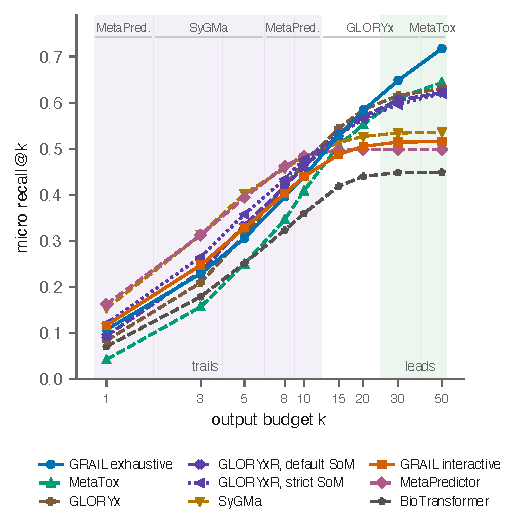
\includegraphics[width=\columnwidth]{fig_sweep}
\caption{Micro recall against output budget on the \numWholeN{} substrates of the whole
evaluated test set. Shading marks the budgets at which the better GRAIL arm trails the strongest
comparator with the paired interval excluding zero (lavender) or leads on the same condition
(green); budgets where neither separates are unshaded. The names along the top give the strongest
comparator over each stretch of budgets, which is the arm the shading there is read against. A
budget here caps a list and leaves its length to the system; Figure~\ref{fig:matched} reads the
same comparison at the length each comparator chose.}
\label{fig:sweep}
\end{figure}

Moving to the larger population costs more cells than it buys: \numPopmoveVerdictsWord{} paired
verdicts change, \numPopmoveHelpedWord{} of them into a separating lead for one of this work's
arms and \numPopmoveNothelpedWord{} not. The wider population narrows every interval, and most of
what that settles at the tight and middle budgets, it settles against us. The headline survives
it: the exhaustive arm separates from all \numWideCompFiveZeroOfWord{} comparators at both of the
widest budgets on either population.

What separates at the tight budgets is an ordering over chemistry the systems share.
\numSygmaInside{} of SyGMa's \numSygmaRules{} published rules sit in this bank verbatim, so SyGMa's advantage
at those budgets is an advantage in ranking: the transformations are shared, and SyGMa orders them
better. On the
comparison set, of the tight-budget cells only the one at $k=1$ survives the family-wise
correction, and it is also one of the three cells the alternative aggregation moves, under which
it does not separate (Table~\ref{SI-tab:si-macro}).

Two further controls apply to the same leads. The first is a family-wise correction, whose reach
is narrower than it sounds. The exhaustive arm leads a comparator in \numSweepWideleadsWord{} cells
at one of the two widest budgets, and the corrected family was declared in advance over
\numSweepFamilycomparatorsWord{} comparators, so the correction covers
\numSweepWideleadsinfamilyWord{} of those cells and leaves \numSweepWideleadsoutsideWord{} outside
it. Of the \numSweepWideleadsinfamilyWord{} it does
cover it removes one: the margin over MetaTox at $k=30$, $+\numMarginMarginalgap$
$[+\numMarginMarginallo, +\numMarginMarginalhi]$. Its lower bound is smaller than the largest
drawing correction measured on any comparator here, $+\numSygdialectThirty$ for SyGMa at the same
budget.

The drawing is the second control, and it is measured on the comparison set, the population
for which the re-run exists. SyGMa met the corpus's form of each substrate, where our declared
standardiser produces another, and re-run on that form the lead holds,
\numMatchedSygmadrawingcost{} narrower over \numMatchedBanksygmastdSlots{} slots
(Table~\ref{SI-tab:si-matched-comparison}). The correction moves one cell the other way: against the corrected
SyGMa the interactive arm's deficit separates, where against the stored drawing it did not.

A recall figure aggregates over transformations of very different kinds, so we read the comparison
class by class as well, at a budget of fifteen and at each comparator's own length
(Figure~\ref{fig:chemistry}, Table~\ref{SI-tab:si-chemistry}). The largest class is
\numChemLargestName{}, \numChemLargestRefs{} of the \numChemReferences{} known metabolites, where the exhaustive
arm recovers \numChemLargestBank{} against \numChemLargestBest{} for the best arm. Where the bank earns its size is cleavages losing two or more carbons, \numChemCleavageRefs{}
known metabolites recovered at \numChemCleavageBank{} against \numChemCleavageBestother{} for the
best comparator. Second by size is the class the vocabulary leaves unnamed, \numChemSecondRefs{}
of \numChemReferences{}, where the best recall any method reaches is \numChemSecondBest{}: a fifth
of the annotated chemistry falls outside what any of the \numChemArmsWord{} systems was built for,
and a headline recall figure hides it. The exhaustive arm trails the best arm on
\numChemBehindWord{} of the \numChemClassesWord{} classes, which carry \numChemBehindrefs{} of the
\numChemReferences{} known metabolites. The two largest of those are \numChemBehindFirstname{} and
\numChemBehindSecondname{}, carrying \numChemBehindTworefs{} between them; the classical small
rows are among them too, demethylation, sulfation, methylation and acetylation carrying
\numChemSmallrowsrefs{} together, read as a direction since none is given an interval. The aggregate advantage is carried by unusual cleavages and by the unnamed
residue.

\begin{figure}[t]
\centering
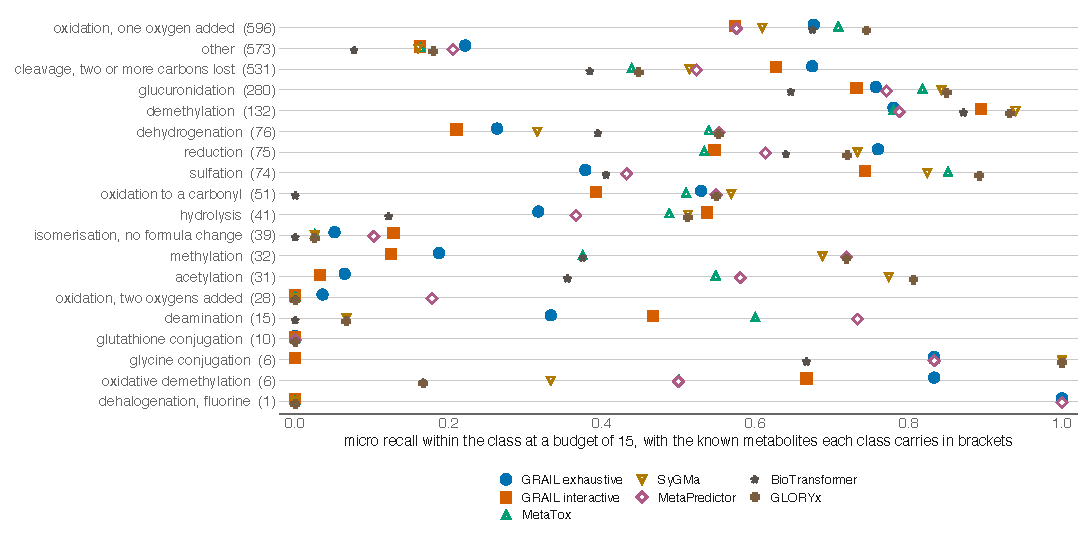
\includegraphics[width=\columnwidth]{fig_chemistry}
\caption{Micro recall within each transformation class at a budget of fifteen, on the comparison
set. Classes run from the one carrying most known metabolites to the one carrying fewest, with
that count in brackets after the name; marks are offset within a class so that systems agreeing to
the digit stay separate. Filled marks are the two GRAIL arms and hollow marks the published
comparators.}
\label{fig:chemistry}
\end{figure}

The one lead that survives all three controls is the exhaustive arm over SyGMa, which makes it an
ordering result on a comparator whose own rules are largely inside this bank. It holds under the
single test SyGMa's own settings allow: at its deeper scenario SyGMa emits more than five times
what the exhaustive arm returns, and the gap does not close.

The lead sits at depth in the list. MetaPredictor is flat from $k=15$ because
\numShortMetapredictorOneFive{} of its \numPopulationN{} lists are shorter than that budget,
SyGMa gains little beyond it, and the exhaustive mode keeps having candidates. Turning
MetaPredictor's beam up narrows the margin at thirty and removes the one at fifteen
(Section~\ref{SI-sec:si-comparators}).

Against MetaTox alone, the deployed system this one succeeds, the exhaustive mode leads at all
\numMtmodeBudgetsWord{} budgets and separates at seven, in the mode its column was submitted in.
The matched-length control removes all seven, and the comparator's other mode removes
\numMtmodeShiftsbankWord{} of the \numMtmodeBudgetsWord{} verdicts
(Table~\ref{SI-tab:si-metatox-mode}).

What a caller receives at a wide budget is mostly wrong, and the cost of the lead is the other
half of it. Table~\ref{tab:si-precision} gives micro precision at every budget: at fifty the
exhaustive arm returns about thirty structures for each annotated one, and no method in the
comparison is far from that. These figures are a lower bound of unknown depth. A structure counted
wrong here may be a metabolite the corpus leaves unannotated, and the corpus alone cannot tell
such a case from a genuine false positive. The order of
magnitude is still the one to plan around: a service answering at that budget hands a chemist a
list to triage. Figure~\ref{fig:pr} puts the two together as the budget sweeps, which is the
shape a ranked list is usually read in: every arm trades precision for recall along one curve,
and the arms that reach furthest right do it at the lowest precision.

\begin{figure}[t]
\centering
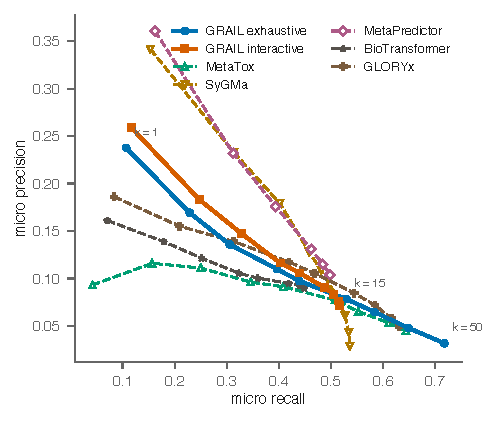
\includegraphics[width=\columnwidth]{fig_pr}
\caption{Micro precision against micro recall on the comparison set, each line one arm traced as
the output budget widens from one candidate to fifty. Filled markers are this work's two arms and
hollow markers the published comparators; three budgets are labelled on the exhaustive arm's
curve. The two GLORYxR settings are absent because the precision table predates them.}
\label{fig:pr}
\end{figure}

\begin{table*}[t]
\centering\scriptsize
\begin{threeparttable}
\caption{Micro precision at each budget on the comparison set, under the parent-drop convention Table~\ref{tab:sweep} uses.}
\label{tab:si-precision}
\setlength{\tabcolsep}{4pt}
\begin{tabular}{rrrrrrrr}
\toprule
$k$ & GRAIL\ exhaustive & GRAIL\ interactive & MetaTox & SyGMa & MetaPredictor & BioTransformer & GLORYx \\
\midrule
$1$ & .2376 & .2590 & .0932 & .3416 & .3608 & .1612 & .1861 \\
$3$ & .1693 & .1832 & .1161 & .2329 & .2319 & .1389 & .1552 \\
$5$ & .1358 & .1472 & .1111 & .1794 & .1758 & .1216 & .1392 \\
$8$ & .1100 & .1165 & .0963 & .1283 & .1309 & .1056 & .1174 \\
$10$ & .0975 & .1060 & .0914 & .1086 & .1151 & .1005 & .1056 \\
$15$ & .0784 & .0906 & .0773 & .0784 & .1042 & .0949 & .0846 \\
$20$ & .0648 & .0833 & .0653 & .0612 & .1041 & .0926 & .0720 \\
$30$ & .0480 & .0765 & .0535 & .0431 & .1041 & .0908 & .0579 \\
$50$ & .0319 & .0713 & .0450 & .0291 & .1041 & .0899 & .0495 \\
\bottomrule
\end{tabular}
\begin{tablenotes}[flushleft]\footnotesize
\item Precision under an incomplete annotation is a lower bound and is not used here to order systems.
\end{tablenotes}
\end{threeparttable}
\end{table*}


\subsection{Sensitivity to the matching criterion}

Whether a predicted structure counts as a known metabolite is itself a choice, so the whole
comparison is recomputed under each criterion we declare, holding the population, the arms, the
ranking and the parent-drop convention fixed. Of the \numCritCriteria{} declared, the grid here
shows the \numCritDefensibleWord{} that answer whether two structures are one compound: the full
InChIKey, the same key with stereochemistry removed, and a tautomer-aware key. Canonical SMILES
equality tests whether two pipelines standardise alike; a Tanimoto of one on a folded fingerprint
merges structures the fingerprint cannot separate. Both are declared and swept, in the Supporting
Information (Section~\ref{SI-sec:si-sensitivity}).

Among the three the verdict is stable, moving at \numCritDefensibleMovedWord{} of the
\numCritBudgetsWord{} budgets (Figure~\ref{fig:criterion}): against the key we report, the
stereochemistry-blind first block moves \numCritVsrefInchinostereoWord{} of them and the full
InChIKey \numCritVsrefInchikeyWord{}. The arm and the comparator
both change across that grid, so a sign on its own leaves open what was compared with what, and
the figure names both.

\begin{figure*}[t]
\centering
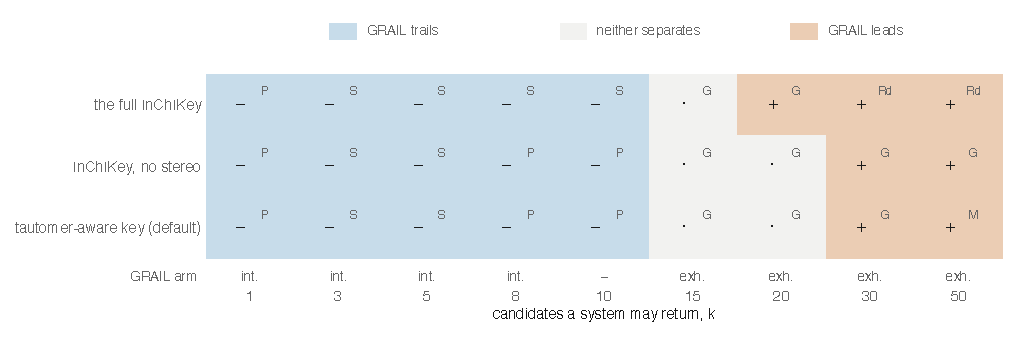
\includegraphics[width=\textwidth]{fig_criterion}
\caption{The verdict of the comparison under each of the three matching criteria this work
reports. $+$ marks a budget where GRAIL's better arm leads the strongest comparator with the
paired interval excluding zero, $-$ one where it trails on the same terms, and $\cdot$ one where
the interval covers zero. The superscript names the comparator the cell is read against, M for
MetaTox, S for SyGMa, P for MetaPredictor, G for GLORYx, and Rd or Rs for GLORYxR in its default
or strict site-of-metabolism setting. The row beneath names the GRAIL arm, \emph{int.} or
\emph{exh.}, with a dash where the better arm is not the same one under all three at that budget.
The two declared criteria this grid omits are in Figure~\ref{SI-fig:si-criterion-all}.}
\label{fig:criterion}
\end{figure*}

At a budget of fifteen the margin between our better arm and the strongest comparator runs from
$\numCritDefensibleWorstOneFive$ to $+\numCritDefensibleBestOneFive$ across the three, a range of
\numCritDefensibleSwingOneFive{} whose sign changes: at that budget the choice among the three
decides the direction.

Taken over all \numCritCriteriaWord{} the verdict moves at \numCritMovedMaxWord{} budgets instead
of \numCritDefensibleMovedWord{}, and the range at fifteen widens from
\numCritDefensibleSwingOneFive{} to \numCritSwingOneFive{}, running from $\numCritWorstOneFive$ to
$+\numCritBestOneFive$. The \numCritLeadsUnderNoIndefensibleWord{} criteria that widen it are
exactly the \numCritLeadsUnderNoIndefensibleWord{} this work leads under at no budget, so most of
the instability a five-criterion sweep reports is its own inclusion. The instability that survives
is on the other axis, the output budget.

The criterion we report is not the one that flatters the result. The tautomer-aware key yields a
lead at \numCritLeadsDefaultWord{} budgets against the \numCritLeadsBestWord{} that
\numCritLeadsbestname{} yields, so a stricter identifier would have given us
\numCritLeadsBestMinusDefaultWord{} more lead than we claim; we chose it because the known metabolites are recorded as constitutions with tautomers merged.

Across the three we report, the comparison leads at
\numCritLeadsUnderEveryDefensibleWord{} budgets under every one of them and trails at the same
\numCritTrailsUnderAnyDefensibleWord{} tight budgets under every one of them.

\subsection{The output budget in an independent benchmark}
\label{sec:external}

The same axis is left undeclared outside this corpus, and there it can be counted. \citet{Gao_2026} deposited the prediction files that the \numExtbudgetArmsWord{}
predictors they benchmarked returned, so what each arm emitted is available directly. Across their
\numExtbudgetDrugs{} drugs the emission spans a factor of \numExtbudgetRatio{}, from
\numExtbudgetNarrowest{} candidates per drug to \numExtbudgetWidest{}, and the arms that emit more
score higher. Shuffling emission among the arms of a single drug, which breaks only which arm is
paired with which emission, loses that association (Section~\ref{SI-sec:si-external}). The spread lives mostly between the arms, which is the level
at which a benchmark orders them. Emission explains part of the ordering and leaves the rest:
ranking the arms by what they emit gives a different order from ranking them by recall, and one
arm returns fewer candidates than another while recovering more.

\subsection{Agreement between the reported site and the observed change}
\label{sec:site}

Every prediction names the transformation rule that produced it and the site at which it fired, so
every candidate carries the mechanistic grounds on which a reader can reject it. Site prediction
is a task with its own literature and its own tools, reactivity-based \citep{Rydberg_2010} and
learned \citep{Sicho_2019, Jacob_2025_uncertainty}, resting on annotation curated for the purpose
\citep{Mazzolari_2019} whose derivation that literature has recently had to confront
\citep{Jacob_2025_autosom}. Our claim is the narrower one that the site this system names is the
site that changed.

We measure that consistency on the interactive arm. Of \numSiteScored{} correctly predicted
metabolites, the reported site touches the atoms that differ from the substrate in
\numSiteTouchingPct{} and lies wholly inside the change in \numSiteInsidePct{}
(Section~\ref{SI-sec:si-site}). The rate on its own overstates the effect, since a site chosen
without regard to the chemistry will sometimes overlap the change by accident; measured
against a connected null fragment of the same size, the margin is \numSiteConnectedmargin{}.

Two things bound the reading. The reference centre is derived by the routine that located the
reaction centre when a template was mined, so for a mined template the two are not independent and
the agreement is partly a self-consistency check. Split by provenance, the hand-written templates
agree at \numSiteCuratedPct{} against \numSiteMinedPct{} for the mined ones, so the claim rests on
the half whose provenance guarantees nothing. The audit runs on the interactive arm alone at a
rule budget of \numSiteRulebudget{}, and the whole bank would score a different population of
matches. What a chemist gets from an attribution also depends on the template:
\numRsizeLethreesharePct{} of parseable templates have three reactant atoms or fewer, and there
the learned stages supply the discrimination between sites.

\subsection{Worked examples}
\label{sec:cases}

\begin{figure*}[t]
\centering
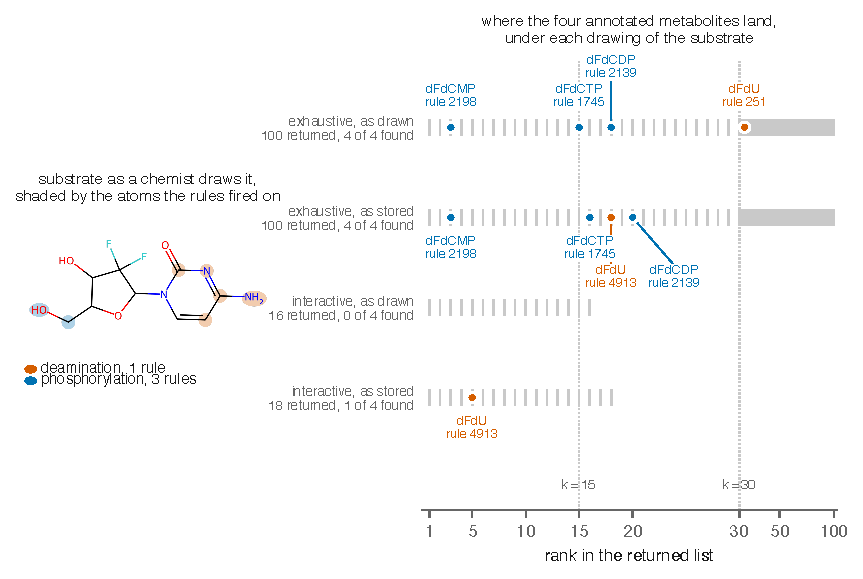
\includegraphics[width=\textwidth]{fig_case}
\caption{Gemcitabine, the second of the two worked examples. Left: the substrate as a chemist
draws it, with each atom a firing rule reported shaded in the colour of its transformation. Right: the rank of each of the
four known metabolites in each arm's returned list, every returned candidate drawn as a tick,
under both drawings of the substrate. The rank axis compresses above $k=30$, where the ticks are
closer together than they are wide and read as a block.}
\label{fig:case}
\end{figure*}

\begin{table*}[t]
\centering\small
\begin{threeparttable}
\caption{Two worked examples: every annotated metabolite of each substrate and the rank the two operating modes return it at, with the bank template that produced it.}
\label{tab:case}
\begin{tabular}{lrrrr}
\toprule
 & \multicolumn{2}{c}{interactive} & \multicolumn{2}{c}{exhaustive} \\
\cmidrule(lr){2-3}\cmidrule(lr){4-5}
annotated metabolite & rank & rule & rank & rule \\
\midrule
\multicolumn{5}{l}{\emph{gemcitabine}} \\
\quad dFdU, deamination & 5 & 4913 & 18 & 4913 \\
\quad dFdCMP, 5$^\prime$-monophosphate & --- & not produced & 3 & 2198 \\
\quad dFdCDP, 5$^\prime$-diphosphate & --- & not produced & 20 & 2139 \\
\quad dFdCTP, 5$^\prime$-triphosphate & --- & not produced & 16 & 1745 \\
\midrule
\multicolumn{5}{l}{\emph{bupropion}} \\
\quad hydrobupropion, carbonyl reduction & 1 & 3065 & 4 & 3065 \\
\quad ring hydroxylation, para to the carbonyl & 3 & 1813 & 1 & 1813 \\
\quad \emph{tert}-butyl hydroxylation, open chain & 5 & 1178 & 10 & 1178 \\
\quad the same, cyclised to the morpholinol & --- & not produced & --- & not produced \\
\bottomrule
\end{tabular}
\begin{tablenotes}[flushleft]\footnotesize
\item Rule is the index into the deployed bank. Both substrates are drawn as the corpus stores them. For gemcitabine that is not how a chemist draws it and the same run on the chemist's drawing returns different ranks, which Section~\ref{SI-sec:si-case} gives; bupropion's stored form is already the standardiser's fixed point, and its two runs are identical.
\end{tablenotes}
\end{threeparttable}
\end{table*}


Two substrates show what each mode returns and what each misses, with the transformation behind
every hit (Table~\ref{tab:case}).

Bupropion is the case the deployed mode handles. The interactive mode returns
\numCaseBupinterCandidates{} candidates in all and places \numCaseBupinterFoundWord{} of the
\numCaseBupReferencesWord{} annotated metabolites at ranks \numCaseBupinterRanks{}: the carbonyl
reduction first, a ring hydroxylation third, and the \emph{tert}-butyl hydroxylation that yields
the major active metabolite fifth. A chemist reading five lines has three of the four. The
exhaustive mode returns \numCaseBupexhCandidates{} and places the same three at
\numCaseBupexhRanks{}, so here the wider pool ranks worse at ten times the reading. Bupropion's
stored form is the standardiser's own fixed point, so its two drawings give identical runs.

The fourth metabolite is instructive. It is the cyclic morpholinol, which is the hydroxylation at
rank \numCaseBupinterDeepest{} closed to a hemiketal: the same molecular formula, and none of the
\numCritCriteria{} declared criteria calls the two equal. The engine produced the chemistry and
the matching rule scored it a miss, which is the axis this paper asks the field to declare,
arriving in a single row.

Gemcitabine is the case it does not. Its four metabolites are the deamination to dFdU that
inactivates the drug and the three sequential 5$^\prime$ phosphorylations that activate it, and
the interactive mode's rule budget never selects the rules that make the phosphorylations, so no
ranking over its candidates could have recovered them (Figure~\ref{fig:case}). The exhaustive
mode produces all \numCaseExhFound{} and reaches every one by rank \numCaseExhDeepest{}, which
is past the budget we report: \numCaseExhPastfifteenWord{} of the \numCaseExhFoundWord{} arrive
only beyond $k=15$, so at the reported budget this molecule counts as one hit of four. It
illustrates the class the bank is weakest on, since at that budget the exhaustive arm recovers
none of the comparison set's \numChemDeamRefs{} annotated deaminations where the best comparator
recovers most of them (Table~\ref{SI-tab:si-chemistry}).

The attribution is what a score cannot supply. All three phosphorylations fire at the same
substrate atoms, the 5$^\prime$ hydroxymethyl, under three different rules, and the deamination
fires on the pyrimidine ring, so the output states which transformation is claimed and where. On
the drawing the corpus stores, all four firing rules are mined, so the part of the bank with no
expert provenance is what carries this molecule. On the drawing a chemist would use, a curated
template finds the deamination instead, and lower in the list
(Section~\ref{SI-sec:si-presentation}).

\subsection{Coverage ceiling of the rule bank}
\label{sec:ceiling}

Applying the whole bank to every test substrate recovers \numCeilingCoverage{} of known metabolites
in a single step, under the criterion the comparison defaults to and on the same evaluated test
set. That is the ceiling any ranking over this bank works under, and what it leaves out is the
subject of this section.

The misses divide by the change each would require at the reaction centre
(Figure~\ref{fig:ceiling}). Most need a transformation type the bank does not hold. A smaller group
needs a type the bank holds whose rule failed to fire, an implementation failure by construction:
three of that group came back once convention-dependent primitives were relaxed, so the group
depends on how the templates are written. A few cannot be typed at all. Of the remainder,
\numContainmentShortfallsharePct{} is of a type the training annotation never holds, measured by a
per-reference join and inside the \numBoundShortfallshareminPct{} to
\numBoundShortfallsharemaxPct{} the cross-tabulation's marginals alone permit
(Section~\ref{SI-sec:si-typeoverlap}).

The distance between the ceiling and what the system reaches divides the same way. On the
comparison set the exhaustive arm at the widest budget reaches \numHeadroomSharePct{} of what the
bank can reach. Of the rest, \numHeadroomRanking{} of recall is headroom a better ranking could
take, and the remaining \numHeadroomCoverage{} would require structures the bank's pool never
contains, so it lies beyond any ranking.

The ceiling is a statement about single steps, and the annotation is not all single steps. Applied
to the known metabolites instead of the templates, our composite instruments flag
\numRefstepEithersharePct{} of the annotated pairs they can type as reached in more than one
turnover and recorded as a single pair. A hit on one of those is a single template standing in for several turnovers, so
\numCeilingCoverage{} is not the share of annotated metabolism that one enzymatic step reaches.

The bound moves with how hydrogen is presented to a template. The count above is measured at the
convention every deployed firing path uses, with hydrogens implicit through the loop a caller runs,
and three other loops differing only in that convention give counts either side of it
(Section~\ref{SI-sec:si-comparators}). All four span \numCeilagreeSpread{} known metabolites, which
is \numCeilagreeSpreadofmarginPct{} of the narrowest margin that separates from zero anywhere in
the comparison, so the choice of instrument cannot decide a claim here. The dependence is real all
the same: measured per template it is $\numHydResidual{}$, 95\% CI $[\numHydResiduallo{},
\numHydResidualhi{}]$, an interval excluding zero.

\begin{table*}[t]
\centering\small
\begin{threeparttable}
\caption{The novel-type gap against the definition of a type.}
\label{tab:grain}
\begin{tabular}{lrrrl}
\toprule
definition of a type & types & once & mass & names a \\
 & & & & transf. \\
\midrule
multiset of changed bonds, with counts & 312 & 294 & 87.2\% & yes \\
the same, counts dropped & 284 & 247 & 73.3\% & yes \\
element pairs that take part & 69 & 30 & 8.9\% & \textbf{no} \\
number of bonds that change & 44 & 9 & 2.7\% & \textbf{no} \\
\bottomrule
\end{tabular}
\begin{tablenotes}[flushleft]\footnotesize
\item Each row is one definition, coarsening downward. \emph{types} is how many distinct types the misses of absent type collapse into under it, \emph{once} how many of those are seen exactly once, and \emph{mass} the share of the gap those once-only types carry. The last column says whether a type under that definition still determines a product. The tail is present wherever it does and collapses only below that.
\end{tablenotes}
\end{threeparttable}
\end{table*}


\begin{figure*}[t]
\centering
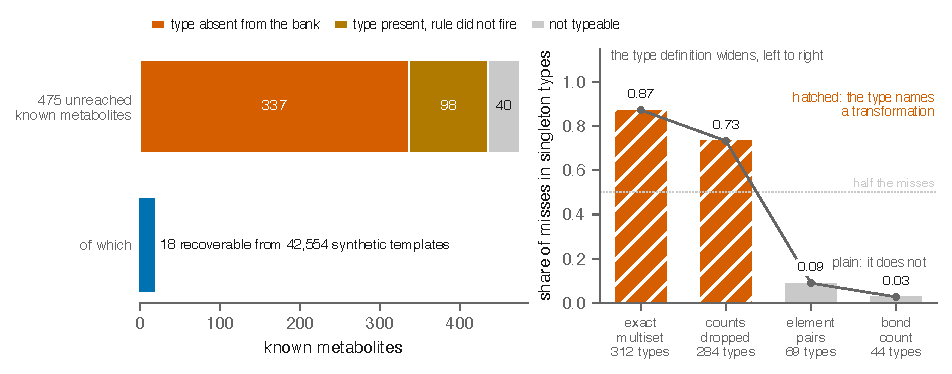
\includegraphics[width=\textwidth]{fig_ceiling}
\caption{Left: where the \numCeilingUncovered{} uncovered known metabolites go, and how many of them a
library of \numUsptoTemplates{} synthetic templates could supply. Right: the share of the
novel-type gap sitting in types seen exactly once, against four definitions of a type; the label
above each bar is that share and the count under each tick is how many distinct types the
definition yields. The hatched bars are the definitions under which a type still names a transformation, so the
distinction does not rest on colour.}
\label{fig:ceiling}
\end{figure*}

The missing chemistry lies in a long tail. The misses of absent type collapse into distinct types
of which those seen exactly once carry \numCensusOnceSharePct{} of the mass, and that tail holds at
every granularity at which a type still determines a product, collapsing only where it stops doing
so (Table~\ref{tab:grain}, Figure~\ref{fig:ceiling}). The share is read under our own definition of
a type and a coarser definition collapses it, which makes the census a fact about how the test
split is annotated; Section~\ref{sec:scope} treats the training annotation separately, and the
engine's contribution is the hydrogen convention measured above. What the census covers should be
said exactly: the misses of absent type, and it does not cover the others.

Nor is the missing chemistry available in the largest reaction library we hold. Typing
\numUsptoTemplates{} retrosynthetic templates \citep{Maziarz_2025, Tanovic_2026} in the metabolic
direction supplies \numUsptoMass{} of those misses. The intersection with the bank is thin,
\numUsptoSanity{} of its \numBankTypes{} types, so that figure is a looser statement than it looks.

\section{Discussion}
\label{sec:discussion}

\subsection{Where the advantage lies}

The comparison does not produce a winner, and the one wide-budget lead that survives every
control is against the comparator whose rules this bank largely contains.

SyGMa's lead at the tight budgets is a result about the field, which this system only inherits.
SyGMa is the oldest and by far the smallest method in the comparison, \numSygmaRules{} published
rules against this bank's \numBankRules{}, and at every budget of five or fewer it recovers more
known metabolites than any other method here, two of them published since. A chemist reading a
short list is working at exactly those budgets. A single recall figure at a single budget would
have named a different winner depending on which budget its author chose, and every one of those
choices would have been defensible.

\subsection{Choosing an operating point}
\label{sec:offers}

The budget a service answers at decides the mode. Below about ten candidates the interactive
mode is the right setting and the faster.

Beyond a short list it is the weaker setting, and the cause is the pool, whose size bounds what
any ranking can return. It returns far fewer candidates than MetaTox and many of its lists have
ended by twenty; a list that has ended stays as it is when the window widens, so the
interactive mode trails MetaTox at every budget above fifteen with the interval excluding zero. A service deployed in that mode would recover less than the
system it replaces wherever it answers with thirty candidates or more, if that system answers in
the mode this column was submitted in. Against its default mode the deficit becomes a lead at
\numMtmodeTrainedreversedWord{} budgets, that mode emitting \numMtmodeEmitteddefault{} candidates
per substrate against \numMtmodeEmittedsmirks{} and ending by fifteen.

A service answering with thirty or fifty candidates must run the exhaustive mode, which leads
MetaTox at both, or raise the rule budget, the knob the exhaustive mode turns to its limit and
which on validation pays only from an output budget of thirty. Either way it pays in runtime and
in what a caller receives, the precision of Table~\ref{tab:si-precision}.

The aggregation was chosen in the direction this paper's result favours. Validation prefers
a blend that discounts duplication up to a budget of \numAggvalHybridwinsmaxWord{}; the released
noisy-or is ahead of it only at the two widest, where the lead reported here is read. The blend
would give a chemist reading a short list more and cost that lead, and re-measuring under it is
left undone (Section~\ref{sec:limitations}).

\subsection{Distinctive properties}

This system reports a site, as the others do: BioTransformer names the reaction and the enzyme
behind each structure it returns, MetaTox's method reports a biotransformation type and a site of
metabolism \citep{Rudik_2017}, and \numArmreturnOrderingWord{} of the \numComparatorsNWord{}
comparators order their whole output. What this work adds is the check in Section~\ref{sec:site}:
the site is read against the atoms that actually changed and against a null of the same size, and
that check appears to be new to this literature.

\subsection{What the measurements establish, and what they leave open}

GRAIL does not lead at the tight budgets. The comparison admits systems that run as released, which
excludes the 2025--26 wave: of the \numComparatorsUnavailableWord{} such systems, every one ships
something short of a runnable metabolite predictor \citep{Larsson_2025, Zhou_2025, Zhou_2026,
Chavan_2026}, and one released weights whose reaction module was later withdrawn. No ranking in this literature can presently be verified
independently, which is the concrete case for leaderboards releasing per-item predictions rather
than aggregate scores \citep{Rodriguez_2021, Mishra_2021}. Precision figures are bounded by
annotation completeness. The advantage at wide budgets is partly a statement about output
length on all sides, independent of ranking.

This paper turned its argument about other people's figures on its own release, and found settings
that decide a number and had gone undeclared: the aggregation of the templates reaching one
candidate, the fusion constant, a rule gate the released checkpoint carries, a set of pools scored
by a checkpoint since withdrawn from this repository, the drawing of the substrate, and the pool
cap.
Each is declared and measured here. The same discipline turned on the comparators finds one more,
and it is this paper's rather than anybody else's: MetaTox exposes a choice of mode to a submitter,
both were submitted, and for two revisions this paper printed one of them without saying which. It
is named and swept here, and the sweep moves \numMtmodeShiftsbankWord{} of the
\numMtmodeBudgetsWord{} verdicts for the exhaustive arm and all \numMtmodeShiftstrainedWord{} for
the interactive one, leaving the lead this paper claims, at budgets \numMtmodeWidebudgets{},
standing under both.

\subsection{Scope of the coverage bound}
\label{sec:scope}

The shortfall is a property of the corpus the templates are mined from, so extending coverage
requires new reaction corpora, and the census narrows the search.
Synthetic corpora are excluded by measurement, which leaves enzymatic and regulatory sources. The
regulatory ones are the interesting half: metabolite identifications from radiolabelled human ADME
studies are human \emph{in vivo} data on exactly the population predicted here, they have been used
to benchmark this class of tool \citep{Gao_2026}, and mining them systematically as a source of
rules is, to our knowledge, still open. Whether the same bound holds for a sequence model, which
works without a template bank, is an open question.

What the bound licenses has to be said plainly, because the corpus it is a property of has two
defects this paper also reports: its assembly cannot be reconstructed, and the one source held on
disk shows the selection was made with chemistry in view. The bound therefore says one thing:
mining the training split harder leaves the shortfall where it is, because that chemistry is
absent from it. Its scope stops there. Stating what fraction of human metabolism lies in types
every corpus omits would need a corpus whose assembly is recoverable and whose selection is
documented.
The narrower statement still earns its place, because this corpus is assembled from the four
sources this field trains on, so a bank mined from any of them inherits the same absence unless the
assembly is changed. The claim is about a training corpus and about the practice of mining it, not
about metabolism.

\section{Limitations}
\label{sec:limitations}

Applying one template once is not the same as one enzymatic step. Applied to the templates, the registered instrument flags
\numCompositeEditsharePct{} of the mined ones it can score as composite, clearing the bar
registered beforehand. A second instrument flags a smaller share and errs in both directions with
both errors unmeasured, so its figure is an estimate of unknown sign
(Section~\ref{SI-sec:si-singlestep}). The ceiling is therefore a one-template one where a single
enzymatic step may take several, and that share is why a second application buys little: a
depth-two probe put the lift at \numDepthtwoLift{} at \numDepthtwoCost{} times the cost.

Two registered mechanisms failed: emitting candidates in whole groups, and gating on the group
signal before the fusion. An oracle closes the second, since even a perfect ordering through it
is worse than the generator cap it replaces (Section~\ref{SI-sec:si-oracle}).

Both learned stages are trained short of what the split allows, on a subsample, and the runs ended on their epoch budget with early stopping unused, an underfitting signature; retraining on the full split is
left to future work (Section~\ref{SI-sec:si-retrain}). One checkpoint produced every figure, so the
intervals quantify the population with training held fixed. Against the noise
\numSpreadSeedsWord{} seeds measure, the rank fusion and the pool cap stand well clear of it
and the rule budget sits inside it, which makes that one indicative only.

The register is weaker than its count suggests. Two of the six confirmed predictions clear the
falsification condition only as written, comparing a point estimate to a threshold where the
stricter reading asks the whole interval to clear it: the rank fusion and the pool cap have their
thresholds inside their own intervals, so the data establish only that the effect exceeds zero.
The group score as a third ranking is weaker again, its threshold fixed in advance while its
population was chosen afterwards, on the comparison set, derived from the test split and recorded
after the fact; Table~\ref{tab:hyp} records that as a measurement, which leaves six.

Every method runs out of candidates at wide budgets, so the widest columns measure list length as
much as ordering; the bound annotation completeness puts under precision is in
Section~\ref{sec:results}. The comparison set is a quarter of the evaluated test split, and the rule
by which it was drawn went unrecorded (Section~\ref{SI-sec:si-population}).

Two comparators are built on sources this corpus is assembled from, which favours both and is left
uncorrected: BioTransformer on MetXBioDB, GLORYx against the reference set of the same name.
A correction would need a model of how much of a rule set a reference set produced, which is
beyond this work, but the bound is measured and small: \numSrccovTraced{} of the \numSrccovPairs{}
annotated pairs carry a transformation either source also records, \numSrccovSharePct{}, on a
match loose enough to count generously (Section~\ref{SI-sec:si-corpus}), so whatever those two
gained they gained on at most that fraction. For the remaining three the overlap is unknown rather than zero, since MetaTox and
MetaPredictor publish no development set to intersect with this corpus.

Validation prefers the aggregation of Section~\ref{sec:offers} over the deployed one, and the
deployed one is the one under which the lead reported here stands. The blend's margin on
validation has its interval clear of zero (Section~\ref{SI-sec:si-aggregation}), selecting it
changes a parameter and leaves the training untouched, and the comparison-set table already
carries it as a column (Table~\ref{SI-tab:sweep-comparison}); re-measuring every figure under it
was priced and left undone. GLORYx is the one arm run elsewhere, because the models it needs ship
separately from its source.

The arms met the substrate at two different drawings. Of the \numChemArmsWord{},
\numChemDrawnstoredWord{} were handed it as the corpus stores it; MetaTox was not, its submission
re-tautomerising \numDialectMetatoxretaut{} of the \numDialectMetatoxn{}. The direction of that difference favours this work, since this
bank's mined half requires the imidic reactant more often than the amide, and this comparator's
service is the one this system replaces. Correcting our own arms instead, which
Section~\ref{SI-sec:si-presentation} measures, answers a different question; the control that
answers this one is a submission the repository carries, the \numMtcorpusN{} substrates whose
two drawings differ. Until those come back, the MetaTox column is read at a
drawing that favours this work by an amount this paper cannot bound.

Depth, too, was met differently by each arm. It is swept for SyGMa and BioTransformer,
whose depth is ours to turn, and the wide-budget results survive both sweeps; the knob stops
short of the output budget.

Nothing in this pipeline is stereochemistry-aware. The standardiser strips configuration, the
criterion ignores it and the annotation carries none, so sulfoxidation, epoxide hydrolysis and
most conjugation are scored as constitutions. That is a restriction on what may be asked of a
metabolite-structure predictor: sulfoxide and epoxide configuration carry the pharmacology of
several drug classes, and a system working at the level of constitution can be asked which
structure an enzyme makes but not which enantiomer. What it costs is left open:
\numStereoSharePct{} of annotated pairs gain a stereogenic element new to the substrate, and the
criterion sweep cannot price a configuration-aware criterion, because every known metabolite here
is recorded without one (Section~\ref{SI-sec:si-sensitivity}).

No measurement of a system here is external. Every figure is measured on one corpus whose only
published reference set is one of its four sources, so a held-out split of it tests the ranking while the
chemistry it is measured on comes from the same four sources. The selection that drew those
records is lost, and the apparatus built on top, which makes every step from the corpus onwards
reproducible, leaves that one step outside it. What can be checked is a rebuild, which the repository reports substrate by substrate, and the
one source held here in full says the selection was made with chemistry in view: the types it kept and
those it dropped are differently distributed (Section~\ref{SI-sec:si-typeoverlap}). The radiolabelled human ADME sets of Section~\ref{sec:offers}
would serve, and measuring a system here on one would need machine-readable structures, where
that benchmark publishes its known metabolites as drawings. Until then the comparison establishes an
ordering within a corpus, which is weaker than a ranking of the methods.

\section{Conclusions}
\label{sec:conclusions}

GRAIL predicts metabolite structures by selecting templates from a bank of reaction rules, applying
them, and ranking the products by a reciprocal rank fusion of two learned scores. How those two
scores are combined mattered more than what produced them: replacing their product with the rank
fusion gained more recall than any architectural change tested here. One application of that bank
reaches \numCeilingCoverage{} of known metabolites in a single step. Most of what remains is
chemistry absent from the training corpus, so enlarging the bank from the same corpus would leave
it there, and every bank mined from the sources this field trains on inherits that gap.

Which predictor leads depends on how a candidate is judged to match a known metabolite and on how
many candidates it may return, and papers in this area declare neither. That is the case for
releasing the grid, and the predictions it is computed from. The next system can be added to it,
and this one can be checked against it.

\begin{suppinfo}

The Supporting Information is available free of charge on the ACS Publications website.

Corpus, splits and leakage audit; what kind of molecules these are; all five matching criteria,
the two the manuscript's grid omits included, and the comparison's sensitivity among them; the parent-drop convention per arm; every candidate count the paper prints; every comparison
difference with its paired interval, at matched list length and under the other aggregation;
precision at every budget and arm; how the substrate is drawn and where that changes a verdict; the rule bank, its
mining and each collection's provenance; what the rule budget buys and two ranking parameters,
swept; four trained variants of the ranking, three on one
frontier and one below it; architecture, training and settings of both learned
stages; whether the site a prediction names is the site that changed; what each method recovers by
transformation class; whether the missing chemistry is the corpus's or the bank's, and whether
template discovery has saturated; how much annotation is one enzymatic step; the sixteen
registered predictions; group ranking and its oracle; the stage ablations; the choice of evaluation
population; the worked examples on both drawings; runtime methodology; comparator versions and
digests; the evaluation claim against an independent benchmark; provenance and reproduction (PDF)

\end{suppinfo}

\section{Data and Software Availability}

Source code, the deployed checkpoints, the released rule bank, the split manifest, the known
metabolites every recall figure is measured against, the frozen per-substrate predictions of every
arm, the evaluation harness, the provenance sweep and the preregistration with every
hypothesis and its outcome are at \texttt{github.com/doctawho42/GRAIL}, and are available to
reviewers at submission. The train and validation candidate pools are deposited at \ZenodoDoi{}.
The service built on this predictor is MetaTox~3.0 at \texttt{way2drug.com}; it answers in the
interactive mode of Section~\ref{sec:modes}, which is the mode whose deficits this paper reports.

The released bank is not the measured bank. This paper's figures are measured on
\numRelbankMeasured{} templates, of which \numRelbankRemoved{} are also in BioTransformer's
published set; that distribution's licence grants redistribution with attribution and reserves
permission for \emph{commercial} use, so the shipped bank drops them as a courtesy rather than an
obligation and \numRelbankReleased{} ship. The removal is free: every known metabolite those templates
reach is reached by another in the bank. Dropping them from the bank leaves them in
\numRelbankCarriersWord{} of \numRelbankCarrierscanned{} tracked files, which a check reports
file by file. The repository's
licence is \RepoLicence{}, which is the only licence the remaining GPL templates permit, and \texttt{NOTICE.md} carries the decisions file by file.

The corpus, whose four sources and versions Section~\ref{sec:populations} names, is kept out of
the deposit, because ShareAlike and NonCommercial terms cannot both be satisfied by one
derivative; its licence is \CorpusLicence{}. Released instead are the evaluated test substrates
as structures and their known metabolites as the descriptors the matching criteria are decided
by, which lets a reader holding neither licence recompute every recall figure and every cell of
the criterion sweep. A check reports zero disagreements between the two readings. Releasing the
checkpoints is the bar this paper applies to others: a comparison requires weights a reader can
obtain, so one of the \numComparatorsUnavailable{} systems of 2025--26 is excluded here. GLORYxR meets that bar for us and, as yet, for a reader it does not:
its weights were supplied privately for this work, so its two columns stand on sources a reader
can reach only once its authors deposit them, which they intend. Section~\ref{SI-sec:si-comparators}
says so beside those columns and records the digest of every weight file that ran, so the deposit
can be checked against it. Section~\ref{SI-sec:si-corpus} sets out what a reader can rebuild and
the one step that stays outside reproduction.

\section{Author contributions}

N.L.P. designed the system, wrote the code, ran every experiment reported here except the MetaTox
submissions, and wrote the manuscript. A.V.R. ran both MetaTox submissions, in both of the modes
the service offers, reviewed the manuscript and will deploy the released model as MetaTox~3.0 on
\texttt{way2drug.com}.

\begin{acknowledgement}

\Funding{}

\AIUse{}

\end{acknowledgement}

\section*{Notes}

A.V.R. is an author of MetaTox \citep{Rudik_2017}, and the system reported here is released as
its successor on \texttt{way2drug.com}, which also hosts the version it is measured against and
will continue to. The
authors declare no other competing interest, financial or otherwise. The relationship favours this
work: the headline comparison is between two versions of one service, read by the authors of both.
What limits it is on record. Every comparator's per-substrate predictions are frozen and released,
every cell of the grid is printed, and the budgets at which this system trails the version it
succeeds are reported in Section~\ref{sec:discussion} and Section~\ref{sec:limitations}. The
Supporting Information sets out what the MetaTox arm consists of, including the one setting the
service exposes to a submitter that this submission left to it.
